\documentclass{article}
\usepackage[utf8]{inputenc}
\usepackage[spanish]{babel}
\usepackage{fancyhdr}
\usepackage{graphicx}
\usepackage{anysize} %Margen
\usepackage{ragged2e}
\usepackage{float}

\renewcommand{\headrulewidth}{0pt}
 \renewcommand{\tabcolsep}{10mm}

\newcommand\tab[1][1cm]{\hspace*{#1}}
\newcommand{\newsubsection}[1]{
  \indent \textbf{#1}\\
}

\setcounter{secnumdepth}{0}

\pagestyle{fancy}
\fancyhf{}
\fancyhead[L]{Equipo:\tab Ilakech Alakech\\Sistema:\tab[.9cm]PUMA Eventos\\Iteración:\tab[.75cm]Primera\\}
\fancyhead[R]{
\includegraphics[scale=.1]{../imagenes/logo.jpg}}
\fancyfoot[L]{Elaboró:\tab[3cm]Emiliano Galeana Araujo\\Fecha de elaboración:\tab \today\\Versión: \tab[2.8cm] 1.0}

\begin{document}

%% \documentclass{article}
%% \usepackage[utf8]{inputenc}
%% \usepackage{url}
%% \usepackage{hyperref}
%% \usepackage{anysize} %Margen
%% \usepackage{graphicx} %imagenes
%% \usepackage[spanish]{babel}
%% \usepackage[utf8x]{inputenc}

\marginsize{2cm}{2cm}{1cm}{2cm} 
% --------------------------- Carátula --------------------------------
\begin{titlepage}
\begin{center}
{\LARGE \scshape Universidad Nacional Autónoma De México\\
Facultad De Ciencias\\\vspace{10mm} }

%----------------------------------------------------------------------------------------
%   TITLE SECTION
%----------------------------------------------------------------------------------------
\centering

\rule{0.8\textwidth}{.8pt}\\
{\huge \Huge \scshape Ingeniería de Software\\
\vspace{10mm}
\begin{center}

\includegraphics[scale=.2]{../imagenes/logo.jpg}
\end{center}
\textit{ILAKECH ALAKECH}}\\

\begin{center}

\end{center}
%----------------------------------------------------------------------------------------
%   AUTHOR SECTION
%----------------------------------------------------------------------------------------
\vspace{1mm} %5mm vertical space
%% {\huge \scshape Fecha:}\\
\vspace{1mm} %4mm vertical space
%% {\huge 27 de agosto de 2019}\\[1cm]
{\huge \today}\\[1cm]                                     
\vspace{1mm} %5mm vertical space
{\huge Plan de Proyecto}\\[1cm]
\vspace{1mm} %5mm vertical space
{\huge Iteración: 1}\\[1cm]
\vspace{1mm} %5mm vertical space
{\huge Versión: 1.0}\\[1cm]
\vspace{1mm} %5mm vertical space
{\huge \scshape Equipo:}\\
{\Large\itshape Galeana Araujo Emiliano 314032324\par}
{\Large\itshape Macías Gómez Jorge 314318644\par}
{\Large\itshape Segoviano Gómez Víctor Manuel 306255300\par}
{\Large\itshape Torres Bucio Miriam 313284623\par}
{\Large\itshape Velez Cardenas Juan Luis Guillermo 311203987\par}
\vspace{3mm}


\vspace{10mm} %5mm vertical space

\vfill % Fill the rest of the page wit whitespace

\end{center}
\end{titlepage}

%% \tableofcontents

\marginsize{2cm}{2cm}{1cm}{5cm}

\vspace*{9mm}
\begin{center}
  {\LARGE \scshape Especificación de Requerimientos de Software\vspace{10mm} }
\end{center}


\section{Contenido}
Enunciado del Problema\\
\indent Diagrama de casos de uso de la iteración\\
\indent Glosario de términos\\
\indent Detalle de casos de uso de la iteración\\

\begin{itemize}
\item Caso de uso: Visitante
  \begin{itemize}
  \item Prototipo de interfaz de usuario de la iteración.
  \item Casos de prueba de la iteración.
  \end{itemize}
  %% Agregar referencia
\item Caso de uso: Staff
  \begin{itemize}
  \item Prototipo de interfaz de usuario de la iteración.
  \item Casos de prueba de la iteración.
  \end{itemize}
\item Caso de uso: Organizador de eventos
  \begin{itemize}
  \item Prototipo de interfaz de usuario de la iteración.
  \item Casos de prueba de la iteración.
  \end{itemize}
\end{itemize}
\indent \indent Requerimientos no funcionales\\
\newpage


\section{Enunciado del Problema}
Crear un producto de software cuyos objetivos son los siguientes:\\
Un sistema que integre todos los eventos organizador por la Universidad para
facilitar su búsqueda de acuerdo al interés de cada estudiante, y que permita
facilitar el manejo de la asistencia en cada uno de estos.\\
\rule{1\textwidth}{.8pt}\\

\section{Diagrama de casos de uso de la iteración}
\begin{figure}[H]
  \begin{center}
    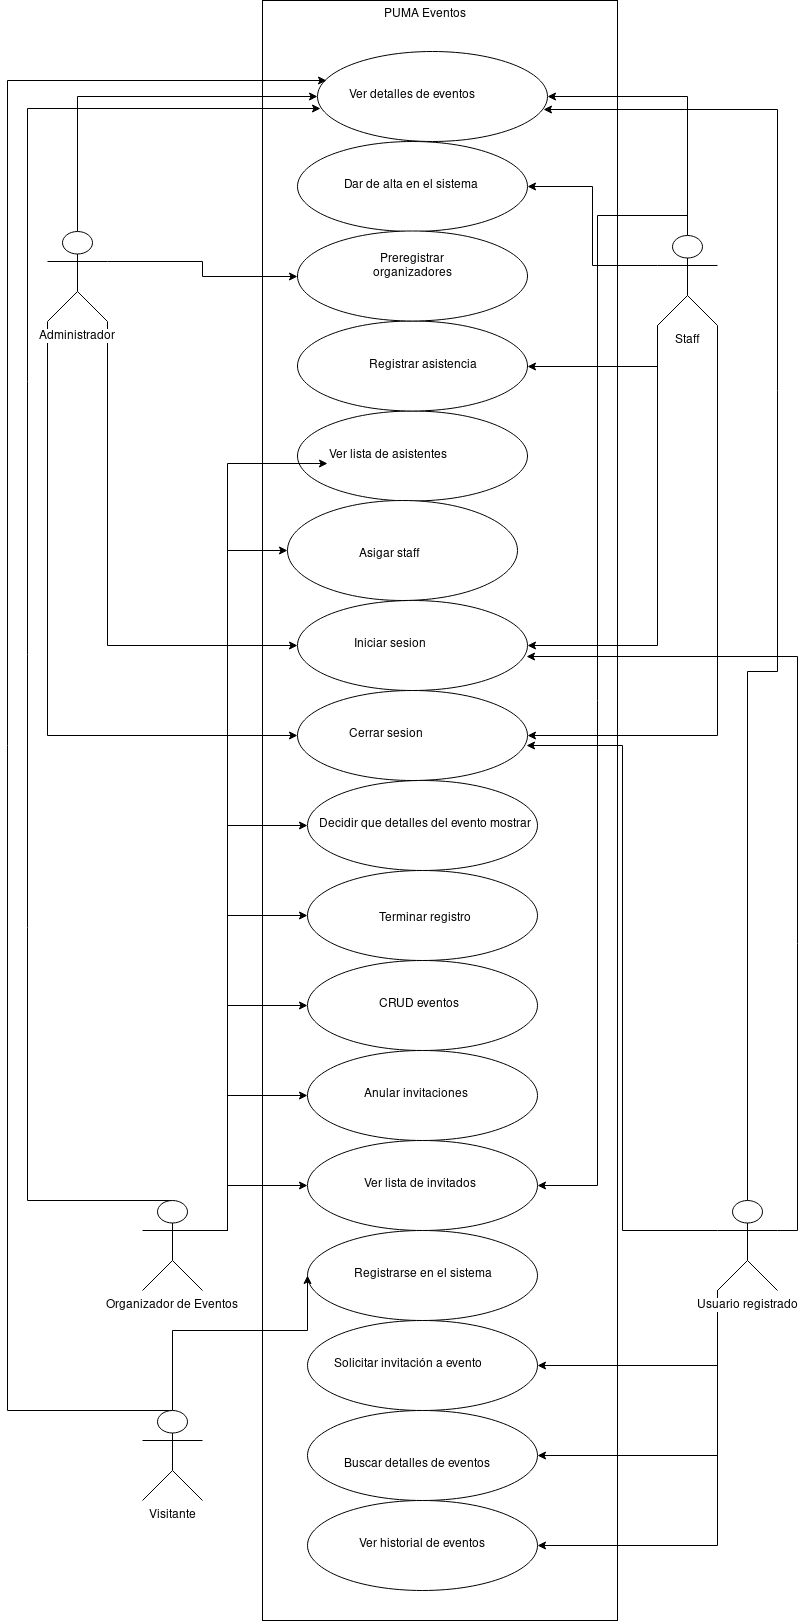
\includegraphics[scale=.3]{../imagenes/diagrama_general.png}
  \end{center}
  \caption{Diagrama general de casos de uso de la iteración. Jorge Macías Gómez
    29 de Agosto de 2019}
  \label{fig:diagrama}
\end{figure}
\rule{1\textwidth}{.8pt}\\

\section{Glosario de términos}
\begin{center}
  \begin{tabular}{| c | c |}
    \hline
    Término & Definición \\\hline
    A & Definición \\\hline
    ... & ... \\\hline
    Z & Definición \\\hline
  \end{tabular}
\end{center}
\rule{1\textwidth}{.8pt}\\

\section{Casos de uso detallados, prototipos de interfaz y casos de prueba}
\subsection{Caso de uso: Visitante}
Responsable: Miriam Torres Bucio\\
\newsubsection{Detalle del caso de uso}
\newsubsection{Diagrama de caso de uso:}
\begin{center}
  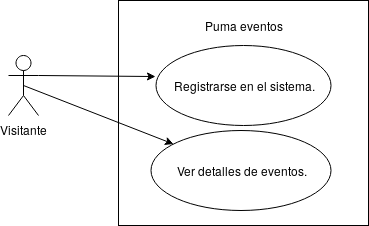
\includegraphics{../imagenes/casoUsoVisitante.png}
\end{center}

\newsubsection{Descripción:}
El visitante puede ver todos los eventos que la UNAM tenga disponibles, puede ver
detalles como fechas, etc., pero no puede buscar eventos ni solicitar invitación
a alguno de ellos, para eso debe de estar registrado.\\
\newsubsection{Precondiciones:}

\newsubsection{Flujo normal de eventos.}
\begin{center}
  \begin{tabular}{| c | c |}
    \hline
    Paso & Acción \\\hline
    1 & El visitante entra al sistema. \\\hline
    2 & El visitante da click sobre el bot\'on de eventos.\\\hline
    3 & El sistema muestra la lista de los eventos disponibles \\\hline
    4 & El visitante puede ver la lista de eventos.\\\hline
  \end{tabular}
\end{center}

\newsubsection{Flujo alternativo de eventos.}

\newsubsection{Flujo excepcional de eventos.}

\newsubsection{Poscondiciones:}

\subsection{Prototipo(s) de las pantallas de interfaz de los casos de la iteración}
Nombre de la pantalla de interfaz 1... % TODO: no entiendo
\subsection{Casos de prueba de los casos de la iteración}
\newsubsection{Casos de prueba (Flujo normal)}

\newsubsection{Casos de prueba (Flujo alternativo)}

\newsubsection{Casos de prueba (Flujo excepcional)}

\rule{1\textwidth}{.8pt}\\
\subsection{Caso de uso: Staff}
Responsable: Emiliano Galeana Araujo\\
\newsubsection{Detalle del caso de uso}
\begin{itemize}
\item Staff.
\item Asistente.
\end{itemize}

\newsubsection{Diagrama de caso de uso:}
\begin{center}
  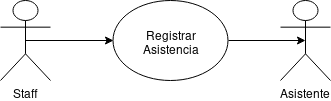
\includegraphics{../imagenes/casoUsoStaff.png}
\end{center}

\newsubsection{Descripción:}
Cuando un usuario asiste a un evento, este necesita mostrar su \texttt{Código QR}
a alguna persona del \textit{staff} para que sea registrada su asistencia.

\newsubsection{Precondiciones:}

\begin{itemize}
\item Que la persona esté registrada.
\item Que la persona sea asistente del evento.
\item Que el asistente tenga en su correo el \texttt{Código QR}
\end{itemize}

\newsubsection{Flujo normal de eventos.}
\begin{center}
  \begin{tabular}{| p{6.9cm} | p{6cm} |}
    \hline 
    Actor & Sistema \\\hline
  \end{tabular}
\end{center}

\begin{center}
  \begin{tabular}{| p{1mm} | c | p{1mm} | c |}
    \hline
    Paso & Acción & Paso & Acción \\\hline
    1 & (Asistente) Mostrar \texttt{Código QR}  & 2 & nada \\
    & en correo & & \\\hline
    3 & (Staff )Leer \texttt{Código QR} & 3 & Verificar
    \texttt{Código QR} \\
    & del correo & & \\\hline
    4 & (Ambos) Esperar & 5 & Mandar un mensaje de\\
    & & & de aceptación o negación \\
    & & & según sea el caso.\\\hline
  \end{tabular}
\end{center}

\newsubsection{Flujo alternativo de eventos.}
\begin{center}
  \begin{tabular}{| c | c |}
    \hline
    Nombre & Acción \\\hline
    Introducir algo que no sea un  \texttt{Código QR}. & Esperar 1 minuto y
    preguntar si se desea intentar\\\hline
    Introducir un \texttt{Código QR} inválido. & Mandar mensaje de código
    inválido. \\\hline
  \end{tabular}
\end{center}

\newsubsection{Flujo excepcional de eventos.}
\begin{center}
  \begin{tabular}{| c | c |}
    \hline
    Nombre & Acción \\\hline
    Error en el servidor al momento de leer el \texttt{Código QR} & Mandar
    mensaje de reintentar. \\\hline
  \end{tabular}
\end{center}

\newsubsection{Poscondiciones:}
\begin{itemize}
\item La asistencia será registrada.
\item El \texttt{Código QR} será puesto como inválido.
\end{itemize}

\subsection{Prototipo(s) de las pantallas de interfaz de los casos de la iteración}
%% TODO

\subsection{Casos de prueba de los casos de la iteración}
\newsubsection{Casos de prueba (Flujo normal)}
\begin{center}
  \begin{tabular}{| c | c | c |}
    \hline
    ID & Entradas & Resultado esperado \\\hline
    N-01 &   
\includegraphics[scale=.2]{../imagenes/qr.png} & Verificado...
    Asistencia Marcada \\\hline
  \end{tabular}
\end{center}

\newsubsection{Casos de prueba (Flujo alternativo)}
\begin{center}
  \begin{tabular}{| c | c | c |}
    \hline
    ID & Entradas & Resultado esperado \\\hline
    A-01 &   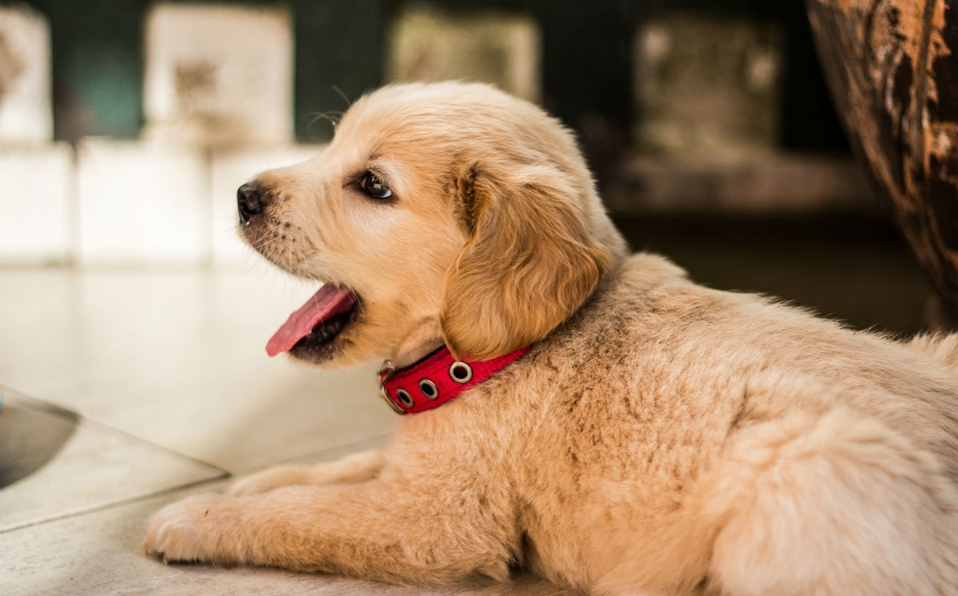
\includegraphics[scale=.1]{../imagenes/perrito.jpg} & No se reconoce
    \\
    & & \texttt{Código QR}, ¿Desea intentar de nuevo? \\\hline
  \end{tabular}
\end{center}

\newsubsection{Casos de prueba (Flujo excepcional)}
\begin{center}
  \begin{tabular}{| c | c | c |}
    \hline
    ID & Entradas & Resultado esperado \\\hline
    E-01 &   
\includegraphics[scale=.2]{../imagenes/qr.png} & No se encuentra
    \texttt{Código QR} \\\hline
  \end{tabular}
\end{center}
\rule{1\textwidth}{.8pt}\\

\subsection{Caso de uso: Organizador de Eventos}
Responsable: Jorge Macías Gómez


\section{Requerimientos no funcionales}
\newsubsection{Interfaz con el usuario.}
\newsubsection{Confiabilidad.}
\newsubsection{Eficiencia.}
\newsubsection{Seguridad.}
\newsubsection{Compatibilidad.}
\newsubsection{Mantenimiento.}
\newsubsection{Portabilidad.}
\newsubsection{Restricciones de diseño y construcción}
\newsubsection{Legales y reglamentarios.}
\end{document}

